\documentclass[12pt,pdftex,a4paper]{article}
\usepackage[english]{babel}
\usepackage{hyperref}
\usepackage{enumitem} 
\usepackage{amsmath}
\usepackage{amssymb}
\usepackage{bbm}
\usepackage[utf8]{inputenc}
\usepackage{float}
\usepackage{cleveref}

\newcommand{\bbN}{\mathbbm{N}}
\newcommand{\bbR}{\mathbbm{R}}
\newcommand{\bbZ}{\mathbbm{Z}}
\newcommand{\bbI}{\mathbbm{I}}

\usepackage{amsthm}
\usepackage{amsfonts}

\usepackage{mathtools}
\usepackage{esvect} % Schöne Vektorpfeile mit \vv{\alpha}
\usepackage[usenames]{color}
\usepackage{polynom}
\usepackage{geometry}
\usepackage{tikz}
\usetikzlibrary{decorations.pathreplacing}
\geometry{verbose,a4paper,tmargin=25mm,bmargin=25mm,lmargin=15mm,rmargin=15mm}
\usepackage{graphicx}
\makeatletter
\def\ScaleIfNeeded{%
\ifdim\Gin@nat@width>\linewidth
\linewidth
\else
\Gin@nat@width
\fi
}
\makeatother

%\geometry{verbose,a4paper,tmargin=25mm,bmargin=25mm,lmargin=15mm,rmargin=20mm}
 
\title{Mathe}

\newcommand{\setN}[0]{\mathbb{N}}
\newcommand{\setF}[0]{\mathbb{F}}
\newcommand{\setR}[0]{\mathbb{R}}
\newcommand{\setZ}[0]{\mathbb{Z}}
\newcommand{\setC}[0]{\mathbb{C}}
\newcommand{\setP}[0]{\mathbb{P}}
\newcommand{\setQ}[0]{\mathbb{Q}}
\newcommand{\setK}[0]{\mathbb{K}}
\newcommand{\winkel}{<\hspace{-1.25ex})\hspace{2.25ex}}
\newcommand{\axi}[1]{{\label{#1}(#1)}}
\newtheorem{defi}{Definition}[section]
\newtheorem{satz}[defi]{Satz}
\newtheorem{prop}[defi]{Proposition}
\newtheorem{koro}[defi]{Korollar}
\newtheorem{lemma}[defi]{Lemma}
\newtheorem*{bsp}{Beispiel}
\newtheorem*{commen}{Bemerkung}
\newenvironment{alphb}{\begin{enumerate}
\def\theenumi{(\alph{enumi})}}{\end{enumerate}}
\newenvironment{arabb}{\begin{enumerate}
\def\theenumi{\arabic{enumi})}}{\end{enumerate}}
\renewcommand{\labelenumi}{\theenumi}
\renewcommand{\theenumi}{\arabic{enumi}.}
\newcommand{\litoinf}{\lim\limits_{n\to\infty}}
\newcommand{\sumtoinf}{\sum\limits_{n=0}^\infty}
\newcommand{\sumtok}{\sum\limits_{n=0}^k}
\newcommand{\sumin}{\sum\limits^\infty}
\newcommand{\fol}{_{n\in\setN}}
\newcommand{\dx}{\mathrm{d}x}
\newcommand{\dt}{\mathrm{d}t}
\usepackage{tabulary}
\usepackage{pdfpages}
\DeclareMathOperator{\Span}{Span}
\let\oldphi\phi
\renewcommand \phi \varphi
\newcommand \my \mu
\definecolor{dunkelgruen}{rgb}{0,0.4,0}


%\usepackage[pdftex]{graphicx}
\usepackage{listings}
\lstset{language=Python,basicstyle=\footnotesize}

\usepackage{newunicodechar}
\newunicodechar{°}{\deg} % \deg wird zum °-Zeichen für Winkel oder Temperaturen. kA, warum LaTeX das nicht direkt mag.


\begin{document}
\title{Bachelor-Forschungsprojekt Informatik:\\Relevante OSM-Tags vorschlagen}
\author{Marco Hildebrand, XXXX, stXXXX@stud.uni-stuttgart.de\\
		Lukas Baur, 3131138, st141998@stud.uni-stuttgart.de\\
		Felix Bühler, 2973410, st117123@stud.uni-stuttgart.de}
\maketitle


\section*{Abstract}
Die vom \textit{Institut für Formale Methoden der Informatik Stuttgart} entwickelte textbasierte Suchmaschine \textit{OSCAR}, die OpenStreetMap-Daten auf Eingabe von OSM-Tags durchsucht, liefert unbefriedigende Ergebnisse auf anderweitige textuelle Eingaben. 
Im Rahmen unseres Bachelor-Forschungsprojekt Informatik sollte diese Lücke geschlossen werden, indem eine Anfrage an das von uns entwickelte System eine Menge an damit verwandten, relevanten Tags zurückgibt.

\pagebreak

\section{Einleitendes}
\subsection{Projektrahmen}
Die Arbeit wurde im Rahmen des \textit{Bachelor-Forschungsprojekts Informatik} in der Zeit vom April bis Oktober 2018 angefertigt. Diese Ausarbeitung stellt die inhaltliche Dokumentation des entwickelten Moduls dar.
\subsection{Initiale Problemstellung}
Grundlage für unsere Arbeit war die Suchmaschine \textit{OSCAR}, die vom \textit{Institut für Formale Methoden der Universität Stuttgart} entwickelt wurde.\\
OSCAR durchsucht auf Eingabe eines \textit{OpenStreetMap-Tags} die  zugehörige Datenbank nach passenden Einträgen und bereitet das Suchresultat grafisch auf. Ein \textit{Tag} ist in OpenStreetMap wie folgt definiert:
\begin{center}
	\textbf{\textit{key}=\textit{value}}
\end{center}
Ein \textit{key} wird benutzt, um ein Themenbereich zu charakterisieren, es repräsentiert einen Typ oder beschreibt ein Feature. Außerdem werden Tags vereinzelt als Namespaces verwendet \cite{keyDescription}.\\
Der \textit{value}-Teil stellt ein Wert des Features da. Typische Werte sind Eigenschaften oder Zahlen \cite{keyDescription}.
Beispiele für Tags sind \textit{building=yes}, \textit{building=house} oder  \textit{highway=service} \cite{example1}\cite{example2}.\\

Da die Eingabe auf Tags beschränkt ist, benötigt ein User zur Suche einen passenden Tag. Diese Lücke soll mithilfe dieses Projekts geschlossen werden. Das zu entwickelnde System soll auf Eingabe eines natürlichen Wortes der englischen Sprache möglichst eng verwandte, relevante OpenStreetMap-Tags vorschlagen.

\subsection{Abgrenzungen}
Unsere Arbeit konzentriert sich auf die Suche der relevanten Tags zu einem eingegebenen Wort. Formaler ausgedrückt besteht unsere Eingabe aus genau einem Wort der englischen Sprache, das nicht in der zugrundeliegenden Stop-Word-Liste enthalten ist.


\section{Projekt-Durchführung}
\subsection{Planungsaspekte}
Zu Beginn unserer Arbeit grenzten wir unser Projekt thematisch ein und überlegten uns eine grobe Vorstrukturierung.
Dazu gliederten wir unser Projekt in \textbf{drei} wesentliche Bausteine:\\
Im zeitlich ersten Arbeitsblock sollten wir uns mit der Darstellung, der Qualität und der Möglichkeit des Zugriffs der Daten vertraut machen. Im Folgenden überlegten wir uns eine aufbereitete brauchbare Daten-Zwischenform, auf deren Grundlage die spätere Suche durchgeführt werden soll. Der dritte Arbeitsbaustein galt der eigentlichen Such-Implementierung.\\
Die bearbeiteten Arbeitspakete werden im folgenden inhaltlich beschrieben. Die Pakete sind intern zeitlich sequentiell beschrieben, überlappen sich allerdings in Ihrer Abarbeitung. Der Grund hierfür sind Abhängigkeiten, wie zum Beispiel, dass die Datenaufbereitung an die Repräsentation des Suchalgorithmus angepasst werden muss, zuvor aber Daten als Grundlage der Suche beschafft sein müssen.

\subsection{Datenbeschaffung}
\subsubsection{Download des OSM Wikis}
Unsere anfängliche Recherche begannen wir mit der Website von OpenStreetMap \cite{WebsiteOSM}, insbesondere mit dem zugehörigem Wiki \cite{WebsiteOSMWiki}. Das OSM-Wiki verfügt über eine ausführliche Dokumentation vieler gängiger OSM-Tags. Unser Ziel war es, auf alle vorhandenen Daten-Tupel, bestehend aus einem gültigen Tag und einer zugehörigen Tag-Beschreibung, lokalen Zugriff zu haben.
\\
Leider bestand nur die Möglichkeit eine veraltete Version des OSM-Wiki von 2013 herunter zu laden, die zudem jedoch frei von erkennbaren Strukturen war, und uns somit keinen Ansatz lieferte. 
\\
\subsubsection{Der Versuch mit tagInfo}
Zwischenzeitlich versuchten wir alternativ mithilfe der Website \textit{taginfo} \cite{taginfoWebsite} an die gesuchten Daten zu gelangen. taginfo wurde in Zusammenarbeit von Jochen und Christian Topf entwickelt und sammelt auf Grundlage der OSM-Daten aktuell rund 2.500 Tags inklusive deren statistischen Charakteristika und teilweise Beschreibungen\cite{taginfoAbout}. Zusätzlich besteht die Möglichkeit, deren komplette Datenbank herunterzuladen.\\
\begin{figure}[h]
	\centering
	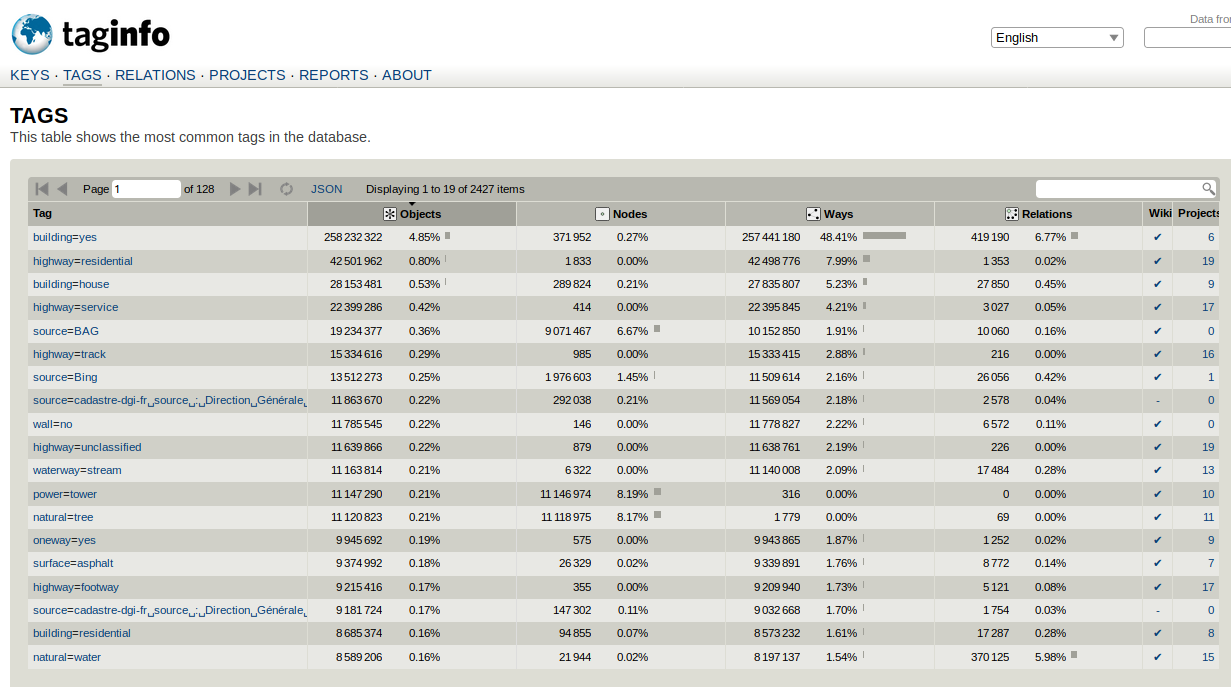
\includegraphics[width=0.9\linewidth]{Bilder/taginfo_example}
	\caption[Beispielhafte Darstellung taginfo]{Beispielhafte Datenbankeinträge der Datenbank von taginfo}
	\label{fig:taginfoexample}
\end{figure}
Leider stellten wir fest, dass die Beschreibungs-Einträge der Datenbank zu lückenhaft und damit für unsere Zwecke nicht geeignet sind.
Als Zwischenlösung kombinierten wir unseren bisherigen Ansätze, indem wir die Tag-Einträge der heruntergeladenen taginfo-Datenbank als Grundlage für ein Crawlen der OSM-Wiki-Seite verwenden wollten: Wir wollten ausnutzen, dass ein Link zu einer tag-beschreibenden Wiki-Seite die folgende Form aufweist:
\begin{center}
	\textbf{wiki.openstreetmap.org/wiki/Tag\%3\textit{Key}\%3D\textit{value}}
\end{center}
Wobei die Variablen \textit{key} und \textit{value} gemäß obiger Erklärung zu füllen sind. Unvorteilhafterweise stellte sich das Downloaden der Seiten schwieriger als gedacht heraus, da es zu manchen Tags noch nicht einmal eine Wiki-Seite gibt.

\subsubsection{Finallösung mit OSM-Wiki-Sitemap}
Schlussendlich verfolgten wir den finalen Ansatz, die aktuelle Sitemap der Wiki-Seiten\cite{sitemap-index-wiki-link} herunterzuladen und anschließend die Links, welche die im vorhergehenden Abschnitt beschriebene Strukur ausweisten, herausgeschrieben.\\
Als Resultat hatten wir nun alle möglichen OSM-Wiki-Seiten lokal im \textit{HTML}-Format zur Verfügung. Es konnten die Daten für den nächsten Arbeitsschritt, dem Aufbereiten der Einträge, weiterverwendet werden.

\subsection{Datenaufbereitung}
Eine Such-Engine auf Grundlage der HTMl-Files aufzusetzen, schlossen wir aus mehreren Gründen aus. Zuerst, findet sich in den HTMl-Files viele unnötige Informationen wieder, z.B. Bild-Links, \textit{JavaScript}-Teile oder gar unwichtige Metainformationen der Seite. Das alles verlangsamt zum einen die spätere Suche, verfälscht zum anderen aber auch den späteren Such- und Indizierungsprozess.\\
Unser Ziel war es, die Daten in eine solche Form umzuwandeln, dass unsere Such-Engine effizient darauf arbeiten kann.

\subsubsection{Initiale Idee}
Zu Beginn verfolgen wir die Idee, wiederkehrende Strukturen zu erkennen und in unser Suchranking miteinbeziehen. Existiert beispielsweise innerhalb der OSM-Wiki-Seite zu dem Tag \textit{highway=residential} ein Paragraphen \textit{related Tags} mit dem Eintrag \textit{highway=tertiary}, so ist es für den Nutzer möglicherweise interessant, auf Eingabe von \textit{highway} beide Ergebisse vorzufinden, auch wenn die Beschreibung von \textit{highway=tertiary} nicht allein zum Suchwort gepasst hätte. Es würde in folge dessen ein Beziehungs-Netzwerk aufgebaut werden.

\subsubsection{Probleme des initialen Ansatzes}
Unglücklicherweise stellten sich heraus, dass die Artikel des Wikis keiner spezifischen Form folgten. Zum einen sind die Strukturen zwischen den Artikeln sehr verschieden (zudem auch verschieden ausführlich), zum anderen finden sich inhaltlich ähnliche Absätze unter verschiedenen Überschriften, so beziehen sich ``See Also'', ``See also'', ``see also'', ``related tags'', ``Related Tags'' oder ``Similar Tag'' eigentlich semantisch auf dasselbe.
Das Ziel, weitere Informationen aus Tabellen zu entnehmen konnte aufgrund der heterogenen Struktur der Seiten ebenfalls nicht erreicht werden.

\subsubsection{Implementierte Variante}
Um die spätere Suchanfrage dennoch befriedigend beantworten zu können, einigten wir uns auf eine Struktur, die die Seite in drei Teile zerteilt. Später werden diese dann unabhängig voneinander durchsucht und gewichtet in die Ergebnisliste eingebracht. Die Struktur der aufbereiteten Daten lässt sich der unteren Grafik \autoref{fig:jsonDarstellung} entnehmen.\\
\begin{figure}[h]
	\centering
	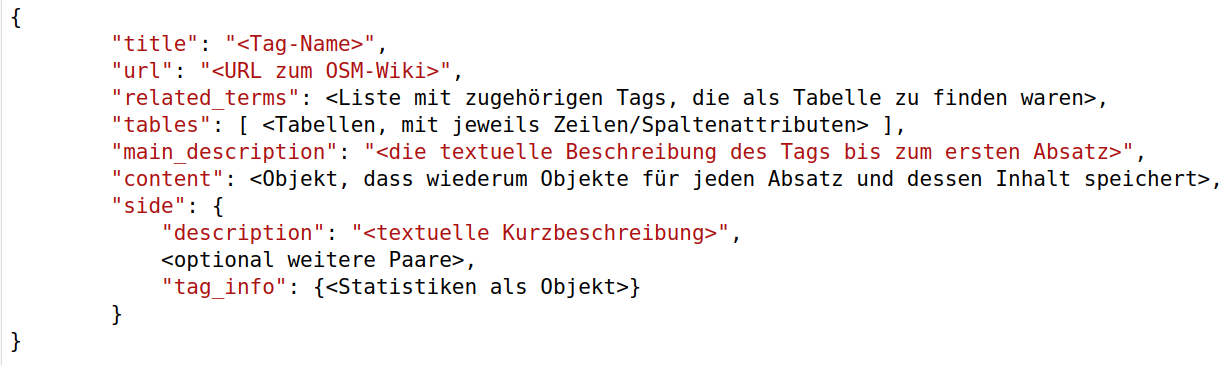
\includegraphics[width=0.9\linewidth]{Bilder/json_structure}
	\caption[Schematische Darstellung]{Schematische Darstellung der \textit{.json}-Struktur. Die Einträge mit spitzen Klammern markieren entsprech Meta-Anweisungen}
	\label{fig:jsonDarstellung}
\end{figure}
Das Ergebnis dieser Arbeitsphase war eine vollständige Liste von \textit{.json}-Objekten, die die texteullen Informationen der HTML-Seiten enthalten, Metainformationen wie Skripte und HTML-Tags jedoch nicht. Zudem sind die Informationen gruppiert und wir erhalten Zugriff auf die Auftrittshäufigkeit eines jeden Tags.

\subsection{Suchanfrage beantworten}



\section{notizen}
Phase 1: Planung
- Tags und dazugehörige semantische Beschreibung holen
- in Struktur bringen
- Suchanfrage an Daten 
    - gensim (Python von Mendel zu Beginn vorgeschlagen)
	- vorhanden/nicht vorhanden 
		-> bewerbung fehlt
	- tf-idf
		-> gut, aber Problem: Mehrere Links auf dieselbe Seite
			-> Duplikate entfernen
		-> hohe Gewichtung für kleine Seiten
			-> Multiplizieren mit log/oder Wurzel 2
- Suchraum expandieren
	- mit Google Modell Anfrage semantisch auffüllen, Suche durchführen, am meisten Relevanten herausnehmen.

\section{ausblick/besser machen}
- Google Modell verkleinern: Wörter raus werfen, damit Modell kleiner wird. Nur Wörter verwenden, die innerhalb des OSM-Wikis vorkommen
- Python NLTK: Entnehme Eingabe Semantische Zusammenhänge: Eingabe von Fragen, Mehrgewichtung gemäß Semantik.
- Extraktion von Schlüsselwörter aus Wiki-Seiten
- Struktur der Seiten besser ausnutzen
	- "nicht zu verwechseln mit .. " wird als treffer gewichtet
	- Tabellen unbeachtet

\section{Einleitung}
\subsection{Projektbeschreibung}

\pagebreak
\section{Vorgehensweise}

1. Anschauen von wiki xml dump (Export von 2013) 
-> Struktur nicht erkennbar + veraltete Daten.

2. taginfo: (um an Tags zu kommen) Datenbank herunter geladen, nicht immer aktuellster Stand, Statitsik: Idee: Generieren von Links, mithilfe von Key=value Anfrage an Website, aber möglicherweise Fehler, da dazu kein Wiki-Eintrag exisitert.

3. nochmal wiki xml dump -> Alle Links des Wikis
4  davon Struktur: filtern der Links, die auf Tags verweisen.
-> Ergebnis: Liste aller Links, die auf OSM-Tag-Seiten zeigen.
5. Crawler: Download aller HTML Files
6. Ergebnis: pretty-Datei.

Implementierung:
1. Schritt: expandieren der Suchanfrage gemäß Semantik auf k Begriffe (mithilfe von W2V) 
2. Schritt: für jeden 


herunterladen der tags: https://taginfo.openstreetmap.org/

\section{Gettings started}
\subsection{languages}
einfach eine liste aller sprachen bekommen mithilfe \texttt{taginfo-wiki.db}.

Die kann man von \texttt{https://taginfo.openstreetmap.org/download} herunterladen.

\subsection{export-links}
herunterladen der osm-wiki sitemap
\texttt{https://wiki.openstreetmap.org/sitemap-index-wiki.xml}


davon interessiert uns nur \texttt{sitemap-wiki-NS\_0-0.xml} der rest enthält daten zu den nutzern, diskussionen und historie

\section{crawl}
alle gesammelten link in die \texttt{links.txt} legen

\texttt{scrapy crawl osmWiki -t json -o keys.json}

\subsection{pretty json}
\texttt{python -m json.tool keys.json > keys-pretty.json}


\pagebreak
\section{Anhang}


\bibliographystyle{unsrt}
\bibliography{lit}

\end{document}